%% ------------------------------------------------------------------------- %%
\chapter{Ajuste dos hiper-parâmetros e normalização em lote}
\label{ape:ajuste-hiper-parametros-cnn}

Neste capítulo apresentamos os resultados dos ajustes dos hiper-parâmetros e da normalização em lote feita nas arquiteturas convolucional, \Gls{unif} e \textit{Embedding}. O intuito destes ajustes é obter um modelo mais robusto e evitar o \textit{overfitting}.

\section{Ajuste dos hiper-parâmetros da rede convolucional}
\label{sec:ajuste-hiper-parametros-cnn}

A rede convolucional exige alguns hiper-parâmetros que devem ser informados durante o treinamento. O tamanho da entrada, conforme citado no capítulo~\ref{cap:experimento}, foi fixado em 150. Caso as palavras tenham tamanho menor, o vetor é preenchido com valores $0$ ao final. Outros três parâmetros exigidos pela rede convolucional são: filtros, kernel e stride.

O parâmetro kernel define o tamanho da janela de operação de convolução. No nosso caso, que estamos utilizando a operação de convolução de 1 dimensão, Conv1D, o kernel define os n-grams a ser extraídos do vetor de entrada. 
O parâmetro filtros define a dimensão de saída da operação de convolução. Este parâmetro indica a quantidade de filtros no resultado da operação de convolução. Cada filtro tenta extrair uma característica diferente do vetor de entrada. E o parâmetro stride define a quantidade de posições de deslocamento do filtro. O parâmetro stride foi fixado em 1. Neste caso, o filtro desloca-se por todas as posições do vetor de entrada de uma em uma posição.

Fizemos alguns testes com relação a quantidade de filtros e o tamanho do kernel utilizando como base os experimentos feitos por \cite{feng-2015} e \cite{tan-lstm-qa}. Tanto \cite{feng-2015} quanto \cite{tan-lstm-qa} utilizaram o parâmetro filtros com o valor entre 1000 e 4000. Em nossos testes, além destes valores, analisamos também os filtros para valores menores como 50, 100, 200 e 500. Já o tamanho do kernel, \cite{tan-lstm-qa} utilizou o valor 2. Em nossos testes, variamos o valor entre 2 e 4, além de concatenar kernels de diferentes valores, combinando kernels de tamanhos 2, 3, 5 e 7.

\subsection{Filtros}

Inicialmente, analisamos o comportamento da rede convolucional proposta no caítulo~\ref{cap:experimento} (ver Figura~\ref{fig:cnn-architecture}) utilizando diferentes quantidades de filtros. Nas figuras a seguir, exibimos um gráfico de comparação do valor do erro no conjunto de treinamento em comparação com o erro no conjunto de validação. Conforme citado no capítulo~\ref{cap:experimento}, foram utilizadas $60.083$ amostras, sendo que $42058$ foram utilizadas para o conjunto de treinamento e $18025$ para o conjunto de validação. Neste experimento, analisamos as seguintes quantidades de filtros: 50, 100, 200, 500, 1000, 2000, 4000. Inicialmente, utilizamos o kernel com o valor 2, valor recomendado por \cite{tan-lstm-qa}.

\begin{figure}[p]
\begin{subfigure}{.5\textwidth}
  \centering
  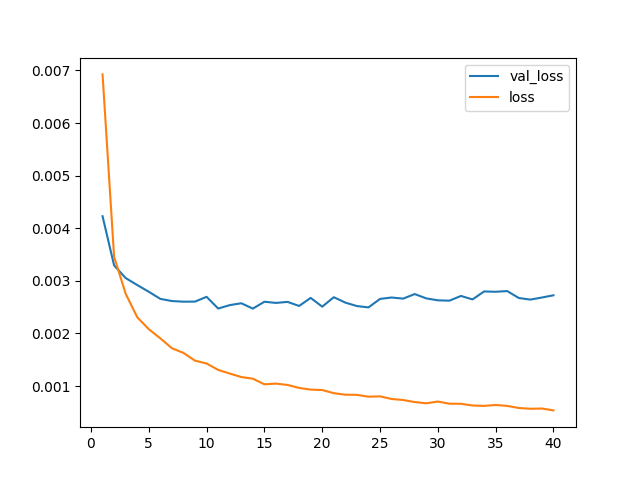
\includegraphics[width=.8\linewidth]{figuras/ape-ajustes-hiper-parametros/cnn-50-k-2.png}
  \caption{Rede convolucional com parâmetro $F = 50$}
  \label{fig:cnn-50-k-2}
\end{subfigure}%
\begin{subfigure}{.5\textwidth}
  \centering
  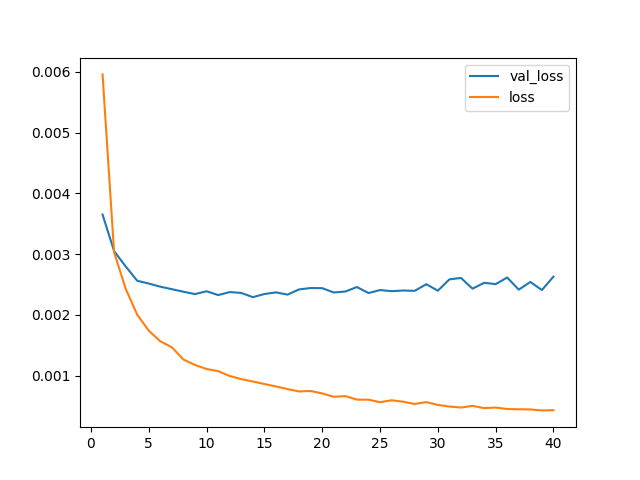
\includegraphics[width=.8\linewidth]{figuras/ape-ajustes-hiper-parametros/cnn-100-k-2.png}
  \caption{Rede convolucional com parâmetro $F = 100$}
  \label{fig:cnn-100-k-2}
\end{subfigure}
\begin{subfigure}{.5\textwidth}
  \centering
  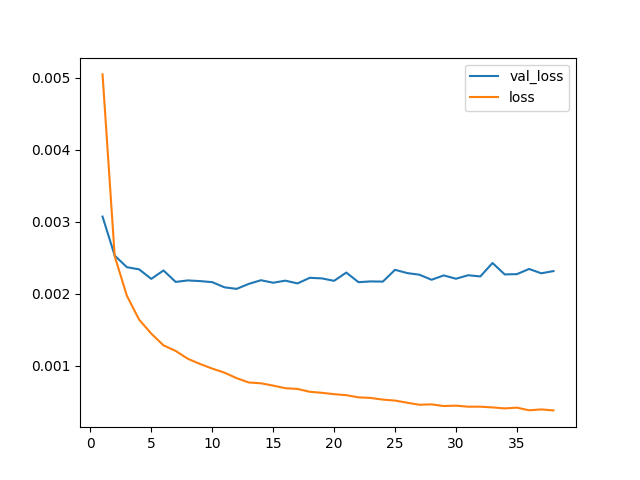
\includegraphics[width=.8\linewidth]{figuras/ape-ajustes-hiper-parametros/cnn-200-k-2.png}
  \caption{Rede convolucional com parâmetro $F = 200$}
  \label{fig:cnn-200-k-2}
\end{subfigure}
\begin{subfigure}{.5\textwidth}
  \centering
  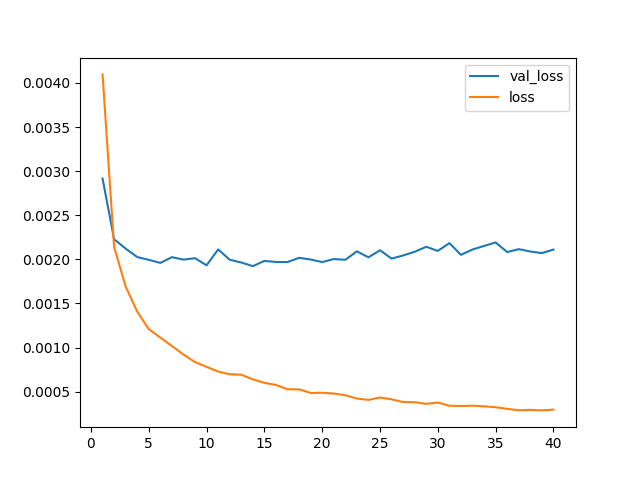
\includegraphics[width=.8\linewidth]{figuras/ape-ajustes-hiper-parametros/cnn-500-k-2.png}
  \caption{Rede convolucional com parâmetro $F = 500$}
  \label{fig:cnn-500-k-2}
\end{subfigure}
\begin{subfigure}{.5\textwidth}
  \centering
  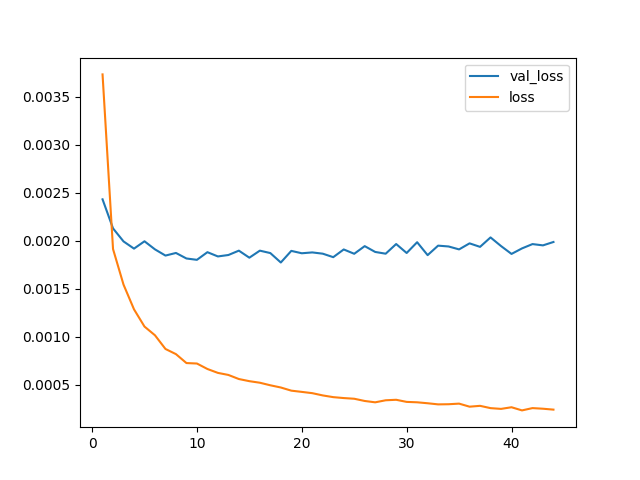
\includegraphics[width=.8\linewidth]{figuras/ape-ajustes-hiper-parametros/cnn-1000-k-2.png}
  \caption{Rede convolucional com parâmetro $F = 1000$}
  \label{fig:cnn-1000-k-2}
\end{subfigure}
\begin{subfigure}{.5\textwidth}
  \centering
  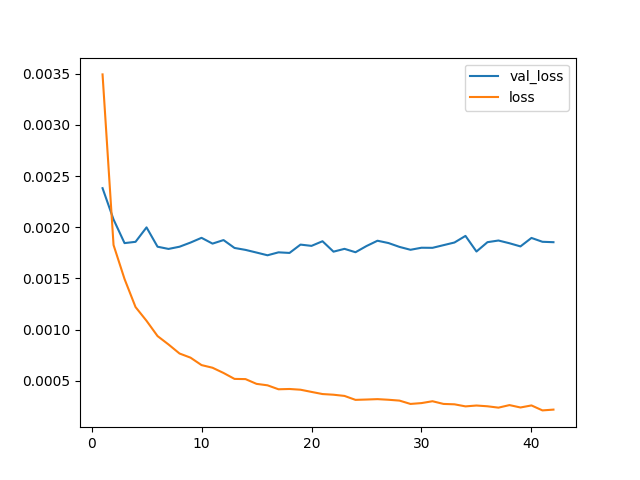
\includegraphics[width=.8\linewidth]{figuras/ape-ajustes-hiper-parametros/cnn-2000-k-2.png}
  \caption{Rede convolucional com parâmetro $F = 2000$}
  \label{fig:cnn-2000-k-2}
\end{subfigure}
\begin{subfigure}{.5\textwidth}
  \centering
  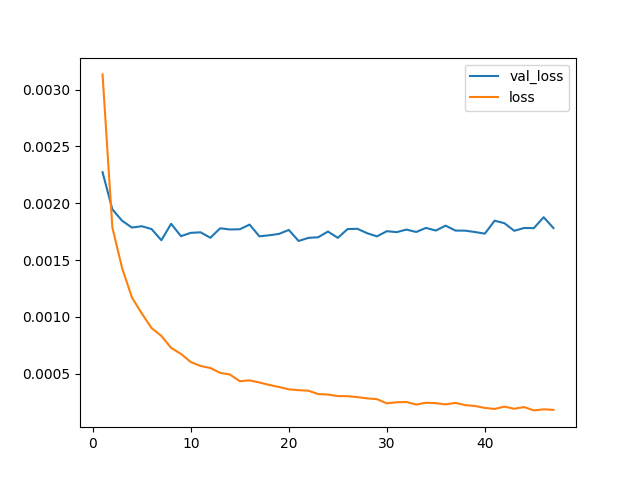
\includegraphics[width=.8\linewidth]{figuras/ape-ajustes-hiper-parametros/cnn-4000-k-2.png}
  \caption{Rede convolucional com parâmetro $F = 4000$}
  \label{fig:cnn-4000-k-2}
\end{subfigure}
\caption{Este gráfico apresenta um comparativo do erro no conjunto de validação em comparação com o erro no conjunto de treinamento. Mais detalhes sobre o treinamento, ver a Seção~\ref{sec:treinamento}. Arquitetura de rede convolucional proposta no Capítulo~\ref{cap:abordagem}, ver Figura~\ref{fig:cnn-architecture}. Hiper-parâmetros: $m = 0.009$, $k = 2$. O parâmetro F indica a quantidade de filtros convolucionais. Nas figuras de \emph{a} a \emph{g}, o eixo \emph{y} indica o valor de erro da função de perda \textit{hinge}, já o eixo \emph{x} indica as épocas de treinamento. A legenda \emph{val\_loss} das figuras de \emph{a} a \emph{g} indica o erro na amostra de validação e a legenda \emph{loss} indica o valor do erro na amostra de treinamento. }
\label{fig:treinamento-cnn-k-2-m-0009}
\end{figure}

De acordo com a Figura~\ref{fig:treinamento-cnn-k-2-m-0009}, o aumento de filtros diminuiu o valor do erro na amostra de validação. O valor de erro que era em torno de $0,003$ na Figura~\ref{fig:cnn-50-k-2}, diminui pela metade, ficando em torno de $0.0015$ nas Figuras~\ref{fig:cnn-2000-k-2} e \ref{fig:cnn-4000-k-2}. O aumento da quantidade de filtros aumenta a capacidade do modelo, pois quanto mais filtros, mais características latentes a rede convolucional tentará extrair dos dados. No nosso caso, isto refletiu no resultado na amostra de validação, diminuindo o valor do erro. Porém, podemos observar que o comportamento do modelo começa a dar sinais de \textit{overfitting}, onde o valor do erro na amostra de treinamento cai abruptamente, enquanto o erro na amostra de validação permance estável e começa a aumentar. Para lidar com este problema, utilizamos normalização em lote e apresentamos os resultados na Seção~\ref{sec:regularizacao-normalizacao-lote}. 

\subsection{Kernel}

Conforme exibido no Capítulo~\ref{cap:abordagem}, o kernel define na rede convolucional de 1 dimensão, o n-grams a serem extraídos. Durante o treinamento, analisamos diferentes valores para o kernel. Verificamos o comportamento para kernel de tamanho 2, 3, 4 e a combinação de valores 2, 3, 5 e 7. Conforme as Figuras~\ref{fig:treinamento-cnn-diferentes-kernels} e \ref{fig:treinamento-cnn-diferentes-kernels-2}, não houve melhora significativa para kernels de tamanho 3 e 4 em comparação com o kernel de tamanho 2. E até mesmo a combinação de kernels não gerou uma melhora significativa dado a quantidade de parâmetros utilizados. Neste caso, optamos por manter o kernel fixado em $2$.


\begin{figure}[H]
\begin{subfigure}{.5\textwidth}
  \centering
  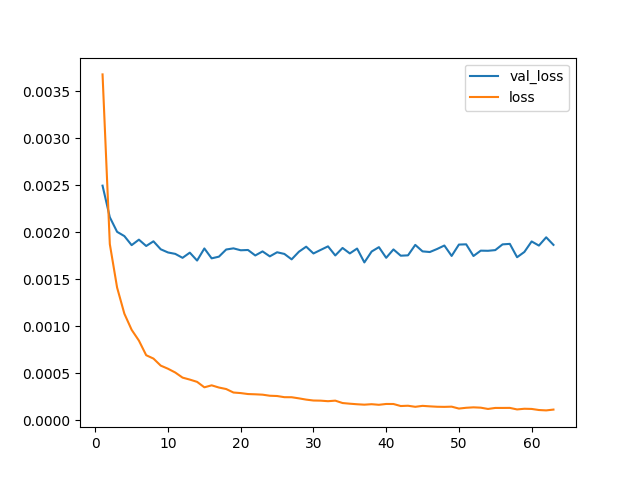
\includegraphics[width=.8\linewidth]{figuras/ape-ajustes-hiper-parametros/cnn-1000.png}
  \caption{Rede convolucional com parâmetros $F = 1000$ e $K = [2,3,5,7]$}
  \label{fig:cnn-1000}
\end{subfigure}%
\begin{subfigure}{.5\textwidth}
  \centering
  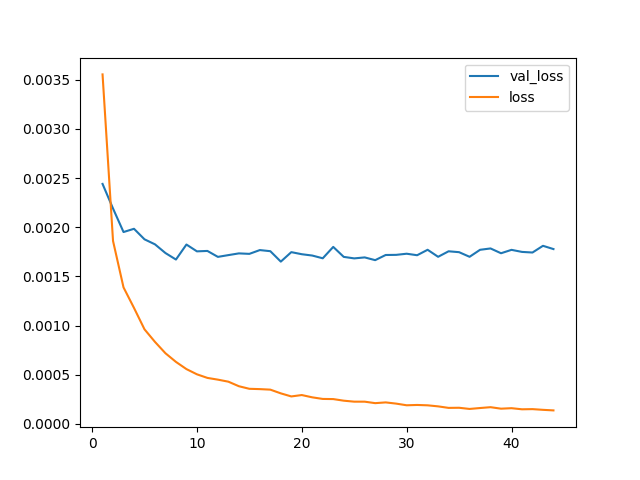
\includegraphics[width=.8\linewidth]{figuras/ape-ajustes-hiper-parametros/cnn-2000.png}
  \caption{Rede convolucional com parâmetros $F = 2000$ e $K = [2, 3, 5, 7]$}
  \label{fig:cnn-2000}
\end{subfigure}
\begin{subfigure}{.5\textwidth}
  \centering
  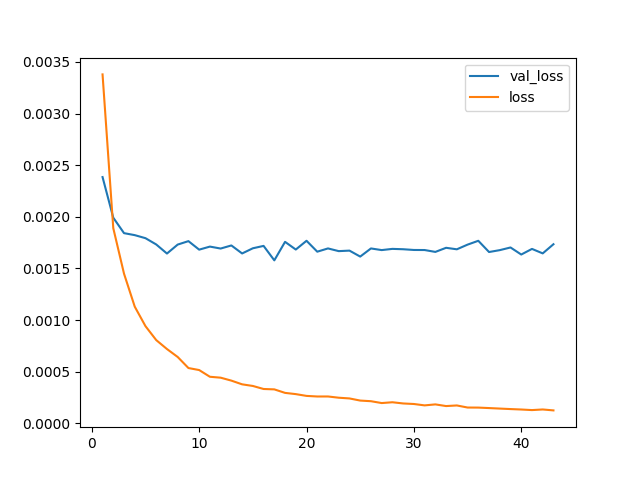
\includegraphics[width=.8\linewidth]{figuras/ape-ajustes-hiper-parametros/cnn-4000.png}
  \caption{Rede convolucional com parâmetros $F = 4000$ e $K = [2, 3, 5, 7]$}
  \label{fig:cnn-4000}
\end{subfigure}
\begin{subfigure}{.5\textwidth}
  \centering
  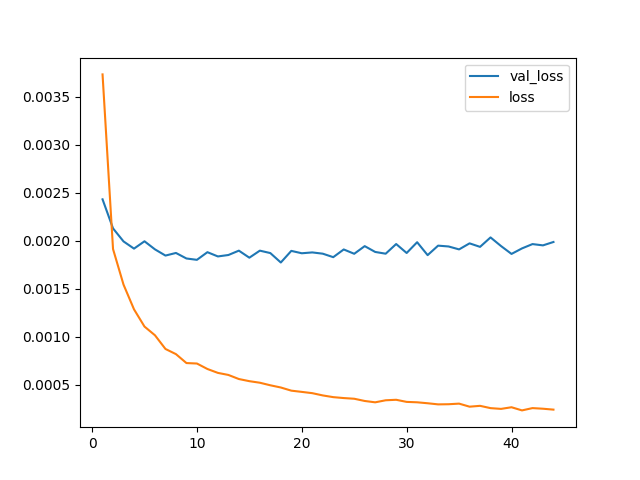
\includegraphics[width=.8\linewidth]{figuras/ape-ajustes-hiper-parametros/cnn-1000-k-2.png}
  \caption{Rede convolucional com parâmetros $F = 1000$ e $K = 2$}
  \label{fig:cnn-1000-k-2-v2}
\end{subfigure}
\begin{subfigure}{.5\textwidth}
  \centering
  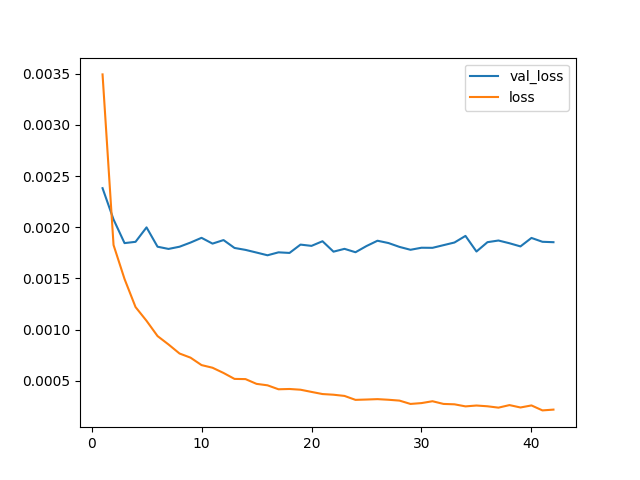
\includegraphics[width=.8\linewidth]{figuras/ape-ajustes-hiper-parametros/cnn-2000-k-2.png}
  \caption{Rede convolucional com parâmetros $F = 2000$ e $K = 2$}
  \label{fig:cnn-2000-k-2-v2}
\end{subfigure}
\begin{subfigure}{.5\textwidth}
  \centering
  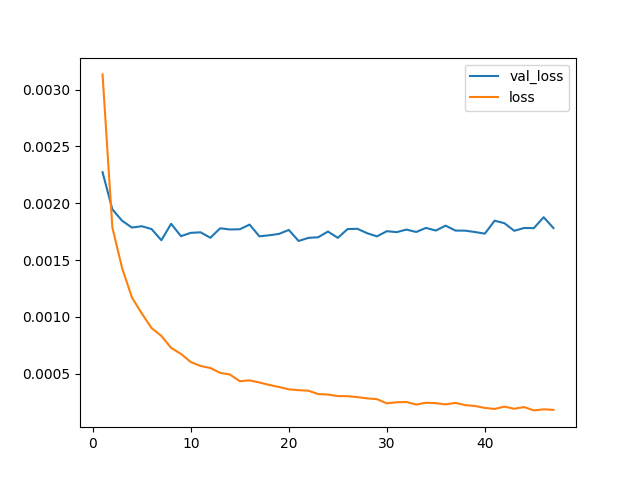
\includegraphics[width=.8\linewidth]{figuras/ape-ajustes-hiper-parametros/cnn-4000-k-2.png}
  \caption{Rede convolucional com parâmetros $F = 4000$ e $K = 2$}
  \label{fig:cnn-4000-k-2-v2}
\end{subfigure}
\caption{Gráfico do treinamento da rede convolucional na recuperação de trecho de código-fonte. Este gráfico apresenta um comparativo do erro no conjunto de validação em comparação com o erro no conjunto de treinamento. Mais detalhes sobre o treinamento, ver a Seção~\ref{sec:treinamento}. Arquitetura de rede convolucional proposta no Capítulo~\ref{cap:abordagem}, ver Figura~\ref{fig:cnn-architecture}. Hiper-parâmetros: $m = 0.009$. O parâmetro F indica a quantidade de filtros convolucionais, o parâmetro K indica o tamanho da janela do filtro convolucional. Nas figuras de \emph{a} a \emph{f}, o eixo \emph{y} indica o valor de erro da função de perda \textit{hinge}, já o eixo \emph{x} indica as épocas de treinamento. A legenda \emph{val\_loss} das figuras de \emph{a} a \emph{g} indica o erro na amostra de validação e a legenda \emph{loss} indica o valor do erro na amostra de treinamento. }
\label{fig:treinamento-cnn-diferentes-kernels}
\end{figure}

\begin{figure}[H]
\begin{subfigure}{.5\textwidth}
  \centering
  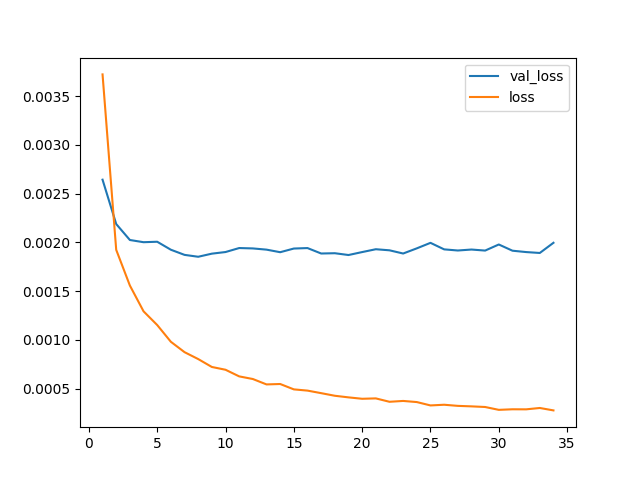
\includegraphics[width=.8\linewidth]{figuras/ape-ajustes-hiper-parametros/cnn-1000-k-3.png}
  \caption{Rede convolucional com parâmetros $F = 1000$ e $K = 3$}
  \label{fig:cnn-1000-k-3}
\end{subfigure}
\begin{subfigure}{.5\textwidth}
  \centering
  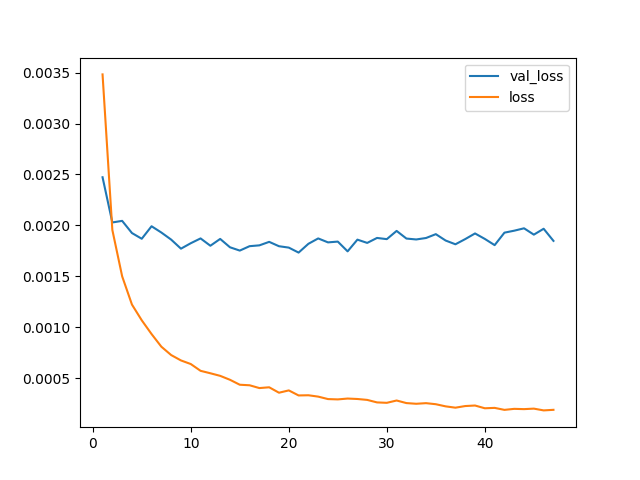
\includegraphics[width=.8\linewidth]{figuras/ape-ajustes-hiper-parametros/cnn-2000-k-3.png}
  \caption{Rede convolucional com parâmetros $F = 2000$ e $K = 3$}
  \label{fig:cnn-2000-k-3}
\end{subfigure}
\begin{subfigure}{.5\textwidth}
  \centering
  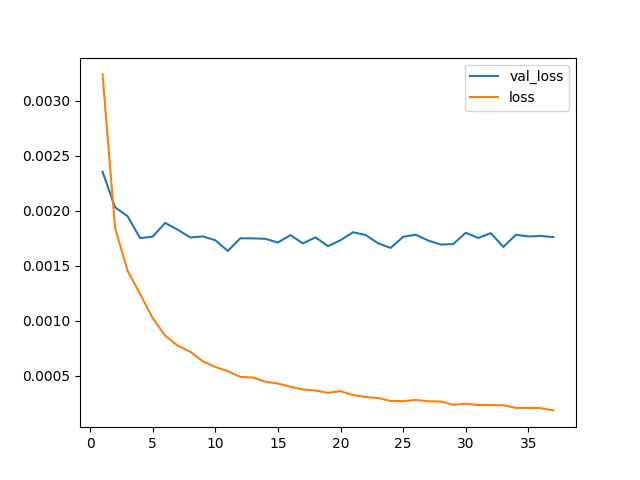
\includegraphics[width=.8\linewidth]{figuras/ape-ajustes-hiper-parametros/cnn-4000-k-3.png}
  \caption{Rede convolucional com parâmetros $F = 4000$ e $K = 3$}
  \label{fig:cnn-4000-k-3}
\end{subfigure}
\begin{subfigure}{.5\textwidth}
  \centering
  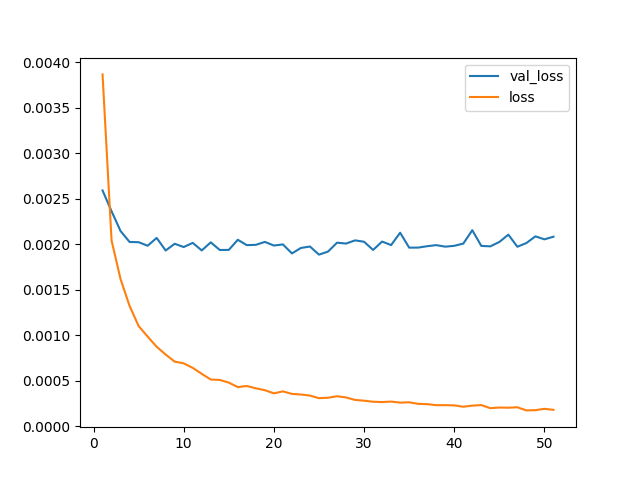
\includegraphics[width=.8\linewidth]{figuras/ape-ajustes-hiper-parametros/cnn-1000-k-4.png}
  \caption{Rede convolucional com parâmetros $F = 1000$ e $K = 4$}
  \label{fig:cnn-1000-k-4}
\end{subfigure}
\begin{subfigure}{.5\textwidth}
  \centering
  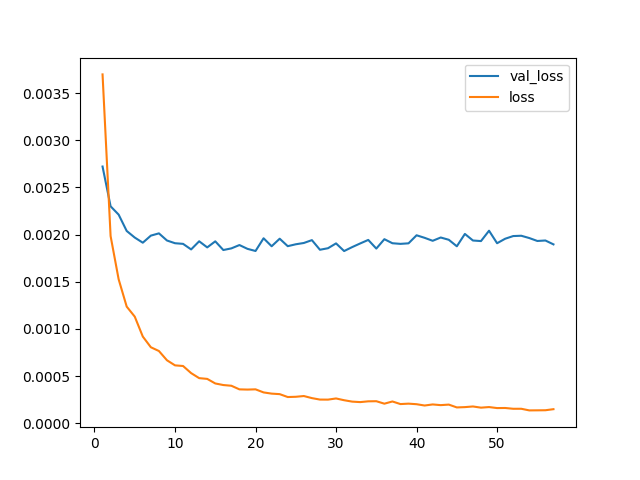
\includegraphics[width=.8\linewidth]{figuras/ape-ajustes-hiper-parametros/cnn-2000-k-4.png}
  \caption{Rede convolucional com parâmetros $F = 2000$ e $K = 4$}
  \label{fig:cnn-2000-k-4}
\end{subfigure}
\begin{subfigure}{.5\textwidth}
  \centering
  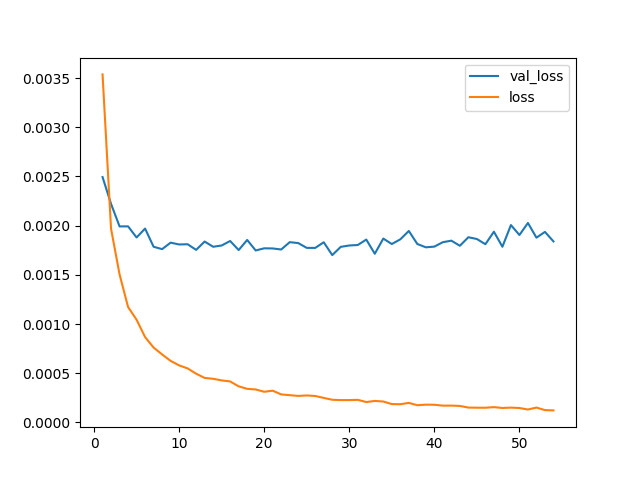
\includegraphics[width=.8\linewidth]{figuras/ape-ajustes-hiper-parametros/cnn-4000-k-4.png}
  \caption{Rede convolucional com parâmetros $F = 4000$ e $K = 4$}
  \label{fig:cnn-4000-k-4}
\end{subfigure}
\caption{Gráfico do treinamento da rede convolucional na recuperação de trecho de código-fonte. Este gráfico apresenta um comparativo do erro no conjunto de validação em comparação com o erro no conjunto de treinamento. Mais detalhes sobre o treinamento, ver a Seção~\ref{sec:treinamento}. Arquitetura de rede convolucional proposta no Capítulo~\ref{cap:abordagem}, ver Figura~\ref{fig:cnn-architecture}. Hiper-parâmetros: $m = 0.009$. O parâmetro F indica a quantidade de filtros convolucionais, o parâmetro K indica o tamanho da janela do filtro convolucional. Nas figuras de \emph{a} a \emph{f}, o eixo \emph{y} indica o valor de erro da função de perda \textit{hinge}, já o eixo \emph{x} indica as épocas de treinamento. A legenda \emph{val\_loss} das figuras de \emph{a} a \emph{g} indica o erro na amostra de validação e a legenda \emph{loss} indica o valor do erro na amostra de treinamento. }
\label{fig:treinamento-cnn-diferentes-kernels-2}
\end{figure}



\section{Ajuste da margem - Função de perda hinge}

Além dos hiper-parâmetros das redes convolucionais, a função de perda \textit{hinge} conforme descrito na Seção~\ref{sec:funcao-objetivo}, exige um parâmetro \emph{margem}. Este parâmetro define a magnitude da diferença da distância de similaridade entre os trechos de código anotados como corretos e os trechos que não são respostas com relação às questões. Os pesquisadores \cite{feng-2015} recomendaram uma margem de $0,009$, enquanto \cite{tan-lstm-qa} utilizaram uma margem de $0,2$. Em nosso caso, fizemos alguns experimentos com os valores $0,009$, $0,05$, $0,1$ e $0,2$. 


\begin{table}[H]
\centering
\begin{tabular}{ p{1cm} p{4cm} P{2.2cm} P{2.2cm} P{2.2cm} P{2.2cm} }
 \hline
    & & \multicolumn{4}{c}{\textbf{Resultados MRR}}\\
 \hline
 & \textbf{Modelos} & \textbf{$m = 0,009$} & \textbf{$m = 0,05$} & \textbf{$m = 0,1$}& \textbf{$m = 0,2$}\\
 \hline
 A1 & Embedding & $0.600$& $0.632$& \cellcolor{Gray!35} $0.637$& $0.635$\\
 
 \hline
 \
 B1 & Unif & $0.647 $ & $0.652$& $0.660$& \cellcolor{Gray!35} $0.674$\\
 
 \hline
 
 C1 & CNN / F = 1000 & $0.654 $ & $0.669$& \cellcolor{Gray!35} $0.676$& $0.637$\\
 
 C2 & CNN / F = 2000 & $0.675 $ & \cellcolor{Gray!35} $0.673$& $0.661$& $0.647$\\
 
 C3 & CNN / F = 4000 & $0.664$ & \cellcolor{Gray!35} $0.687$& $0.672$& $0.651$\\
 
\hline
\end{tabular}
\caption{Resultado da avaliação dos modelos CNN, \Gls{unif} e Embedding na amostra EVAL. MRR refere-se a média do resultado do Mean Reciprocal Rank (equação~\ref{eq:mrr}). O hiper-parâmetro \emph{m} indica a margem utilizada na função de perda \textit{hinge}. F indica a quantidade de filtros convolucionais utilizados durante o treinamento das redes convolucionais. As células destacadas indicam a margem na qual o modelo obteve o melhor desempenho durante a avaliação.}
\label{table:alteracao-margem}
\end{table}



Notamos que não há um consenso sobre o valor da margem, conforme a Tabela~\ref{table:alteracao-margem}, pois cada arquitetura obteve um desempenho diferente para um valor diferente de margem. As redes convolucionais obtiveram o melhor desempenho para uma margem de valor $0,05$, exceto quando a quantidade de filtros convolucionais utilizadas é $1000$. Já a arquitetura Unif proposta por \cite{cambronero-deep-learning-code-search:2019} obteve o melhor desempenho para o valor $0,2$, enquanto a arquitetura \textit{Embedding} obteve com o valor $0,1$. Optamos por fixar estes valores específicos para cada arquitetura, definindo a margem em $0,5$ para a CNN, enquanto para Unif e \textit{Embedding} fixamos em $0,2$ e $0,1$, respectivamente. E conforme descrito na Tabela~\ref{table:alteracao-margem}, escolhemos o valor da margem baseado no valor mais alto da métrica MRR, que foi obtida através da avaliação do melhor modelo na amostra EVAL. Ver a Seção~\ref{sec:avaliacao} para mais detalhes sobre o procedimento de avaliação. 

\section{Regularização - Normalização em Lote}
\label{sec:regularizacao-normalizacao-lote}

Conforme as Figuras~\ref{fig:cnn-1000-k-2-v2}, \ref{fig:cnn-2000-k-2-v2} e \ref{fig:cnn-4000-k-2-v2}, as redes convolucionais estão dando sinais de \textit{overfitting}, onde o valor do erro na amostra de treinamento está diminuindo rapidamente, enquanto o valor do erro na amostra de validação está estável e aumentando ao longo do tempo. Para tentar redimir este problema, aplicamos a normalização em lote para regularizar o nosso modelo. Conforme \cite{sergey-batch-normalization-2015}, a aprendizagem em redes neurais profundas é complicada, pois a distribuição de cada camada é alterada, conforme os parâmetros são atualizados ao longo do treinamento. Isto requer uma otimização e ajuste dos parâmetros a fim de evitar a saturação da função de perda. Para mitigar este problema e auxiliar o modelo a aprender de maneira mais rápida, os pesquisadores apresentaram a normalização em lote, que permite utilizarmos taxas de aprendizagem mais alta e não requer muitos cuidados na inicialização do modelo. Além disso, segundo os próprios pesquisadores, a normalização em lote além de ajudar o modelo a aprender mais rápido, ela auxilia na melhora do desempenho e na obtenção de um modelo mais robusto, não necessitando de outras técnicas de regularização como \textit{dropout} \citep{sergey-batch-normalization-2015}.

Aplicamos a normalização em lote nas redes convolucioanais e de acordo com as Figuras~\ref{fig:treinamento-cnn-normalizacao-em-lote}, podemos notar uma sutil melhora na aprendizagem com a normalização em lote, principalmente para as primeiras 25 épocas iniciais, onde há uma leve diminuição entre o valor do erro na amostra de treinamento em comparação com o erro na amostra de validação. Esta sutil melhora ocorre principalmente para as redes convolucionais utilizando uma maior quantidade filtros, em nosso caso, quando os valores são 2000 e 4000. Esta leve melhora pode ser notada ao comparar as Figuras~\ref{fig:cnn-2000-k-2-m-005} e \ref{fig:cnn-2000-k-2-m-005-normalizacao-em-lote} e também as Figuras~\ref{fig:cnn-4000-k-2-m-005} e \ref{fig:cnn-4000-k-2-m-005-normalizacao-em-lote}.

Podemos notar também que enquanto a normalização em lote auxiliou as redes convolucionais com 1000 e 2000 filtros a tornaram-se mais estáveis (Figuras~\ref{fig:cnn-1000-k-2-m-005-normalizacao-em-lote} e \ref{fig:cnn-2000-k-2-m-005-normalizacao-em-lote}), isto não ocorreu para a rede convolucional com 4000 filtros (Figura~\ref{fig:cnn-4000-k-2-m-005-normalizacao-em-lote}). Mas, ao analisarmos o comportamento da rede convolucional com 4000 filtros, percebemos que as 15 primeiras épocas iniciais, a aprendizagem ocorreu de forma mais estável e somente após a época 25, ocorre um ''grande salto'' e temos uma enorme diferença entre o erro de validação e o erro de treinamento. Para mitigar este problema, adotamos a parada antecipada do treinamento. Conforme explicado na Seção~\ref{sec:treinamento}, caso não haja diminuição do valor do erro na amostra de validação durante 25 épocas seguidas, o treinamento é interrompido e o modelo que obtiver a maior média MRR na amostra DEV é escolhido.

\begin{figure}[H]
\begin{subfigure}{.5\textwidth}
  \centering
  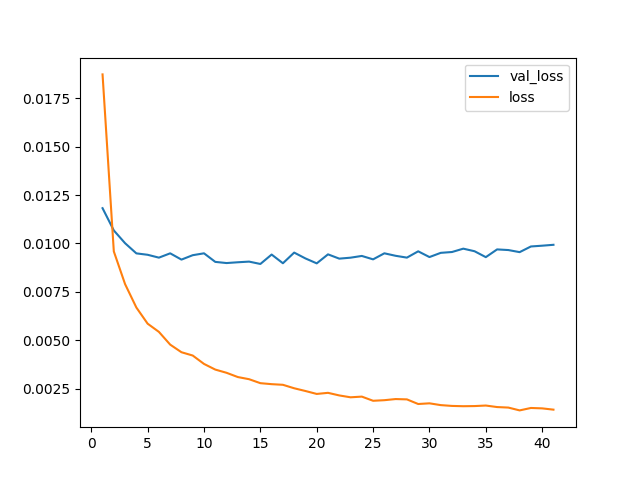
\includegraphics[width=.8\linewidth]{figuras/ape-ajustes-hiper-parametros/cnn-1000-k-2-m-005.png}
  \caption{Rede convolucional com parâmetros $F = 1000$, $K = 2$ e $m = 0,05$.}
  \label{fig:cnn-1000-k-2-m-005}
\end{subfigure}
\begin{subfigure}{.5\textwidth}
  \centering
  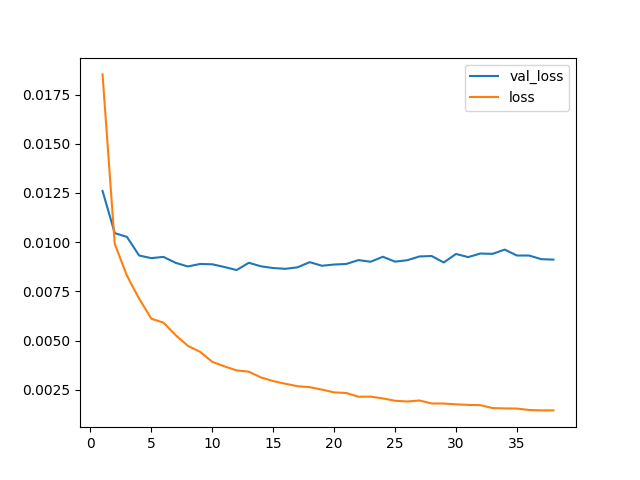
\includegraphics[width=.8\linewidth]{figuras/ape-ajustes-hiper-parametros/cnn-with-bn-1000-k-2-m-005.png}
  \caption{Rede convolucional com parâmetros $F = 1000$, $K = 2$ e $m = 0,05$ e normalização em lote.}
  \label{fig:cnn-1000-k-2-m-005-normalizacao-em-lote}
\end{subfigure}
\begin{subfigure}{.5\textwidth}
  \centering
  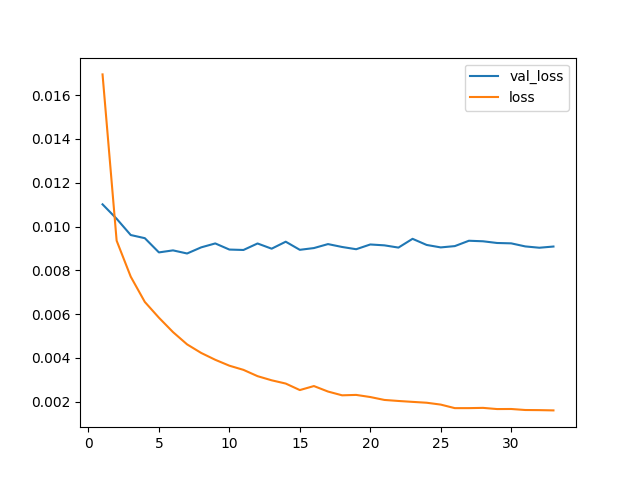
\includegraphics[width=.8\linewidth]{figuras/ape-ajustes-hiper-parametros/cnn-2000-k-2-m-005.png}
  \caption{Rede convolucional com parâmetros $F = 2000$, $K = 2$ e $m = 0,05$.}
  \label{fig:cnn-2000-k-2-m-005}
\end{subfigure}
\begin{subfigure}{.5\textwidth}
  \centering
  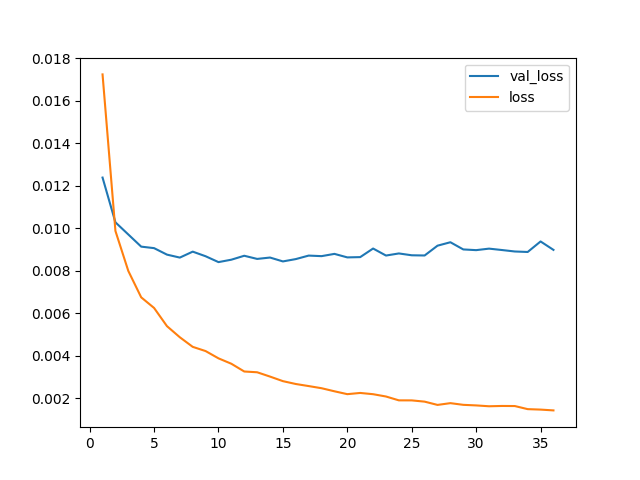
\includegraphics[width=.8\linewidth]{figuras/ape-ajustes-hiper-parametros/cnn-with-bn-2000-k-2-m-005.png}
  \caption{Rede convolucional com parâmetros $F = 2000$, $K = 2$ e $m = 0,05$ e normalização em lote.}
  \label{fig:cnn-2000-k-2-m-005-normalizacao-em-lote}
\end{subfigure}
\begin{subfigure}{.5\textwidth}
  \centering
  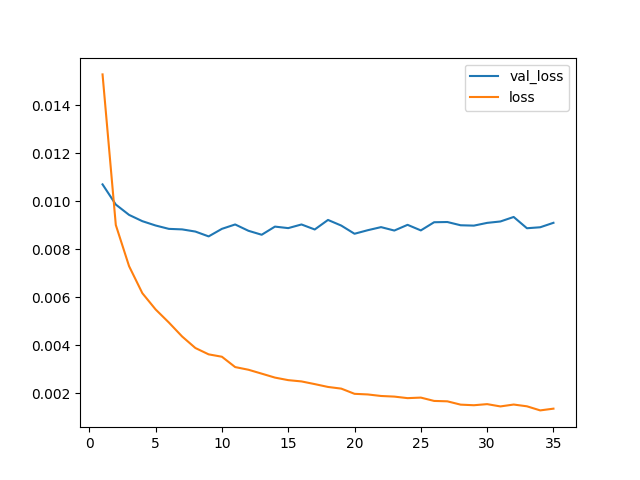
\includegraphics[width=.8\linewidth]{figuras/ape-ajustes-hiper-parametros/cnn-4000-k-2-m-005.png}
  \caption{Rede convolucional com parâmetros $F = 4000$, $K = 2$ e $m = 0,05$.}
  \label{fig:cnn-4000-k-2-m-005}
\end{subfigure}
\begin{subfigure}{.5\textwidth}
  \centering
  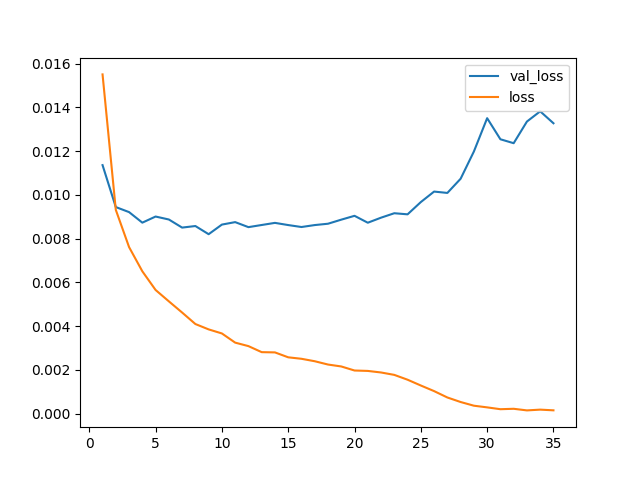
\includegraphics[width=.8\linewidth]{figuras/ape-ajustes-hiper-parametros/cnn-with-bn-4000-k-2-m-005.png}
  \caption{Rede convolucional com parâmetros $F = 4000$, $K = 2$ e $m = 0,05$ e normalização em lote.}
  \label{fig:cnn-4000-k-2-m-005-normalizacao-em-lote}
\end{subfigure}

\caption{Gráfico do treinamento da rede convolucional na recuperação de trecho de código-fonte. Este gráfico apresenta um comparativo do erro no conjunto de validação em comparação com o erro no conjunto de treinamento. Mais detalhes sobre o treinamento, ver a Seção~\ref{sec:treinamento}. O parâmetro F indica a quantidade de filtros convolucionais, o parâmetro K indica o tamanho da janela do filtro convolucional e o parâmetro \emph{m} é a margem utilizada na função de perda \textit{hinge}. Nas figuras de \emph{a} a \emph{f}, o eixo \emph{y} indica o valor de erro da função de perda \textit{hinge}, já o eixo \emph{x} indica as épocas de treinamento. A legenda \emph{val\_loss} das figuras de \emph{a} a \emph{g} indica o erro na amostra de validação e a legenda \emph{loss} indica o valor do erro na amostra de treinamento. Nas figuras do lado esquerdo: \emph{a}, \emph{c} e \emph{e} apresentam o comportamento da rede convolucional durante o treinamento sem utilização de regularização. As figuras do direito: \emph{b}, \emph{d} e \emph{f} apresentam o comportamento da rede convolucional utilizando normalização em lote. }
\label{fig:treinamento-cnn-normalizacao-em-lote}
\end{figure}

Apesar do ''grande salto'' para a rede convolucional com 4000 filtros, a normalização em lote melhorou o desempenho em todas as redes convolucionais. Conforme a Tabela XXX, podemos verificar que houve um aumento do valor do MRR na amostra EVAL. Para nós, isto é um indicativo de que a normalização em lote auxiliou na aprendizagem. Além disso, a parada antecipada impediu o \textit{overfitting} do modelo, permitindo que selecionássemos o melhor candidato à avaliação final na amostra EVAL. Para ter um comparativo nos testes finais, optamos por apresentar os resultados de ambos os modelos, as redes convolucionais com normalização em lote e as redes sem normalização, na Seção~\ref{sec:resultados-avaliacao}.

\begin{table}[H]
\centering
\begin{tabular}{ p{1cm} p{4cm} P{2.2cm} P{2.2cm} P{2.2cm} P{2.2cm} }
 \hline
    & & \multicolumn{4}{c}{\textbf{Resultados MRR}}\\
 \hline
 & \textbf{Modelos} & \textbf{$m = 0,009$} & \textbf{$m = 0,05$} & \textbf{$m = 0,1$}& \textbf{$m = 0,2$}\\
 \hline
 A1 & Embedding & $0.600$& $0.632$& \cellcolor{Gray!35} $0.637$& $0.635$\\
 
 \hline
 \
 B1 & Unif & $0.647 $ & $0.652$& $0.660$& \cellcolor{Gray!35} $0.674$\\
 
 \hline
 
 C1 & CNN / F = 1000 & $0.654 $ & $0.669$& \cellcolor{Gray!35} $0.676$& $0.637$\\
 
 C2 & CNN / F = 2000 & $0.675 $ & \cellcolor{Gray!35} $0.673$& $0.661$& $0.647$\\
 
 C3 & CNN / F = 4000 & $0.664$ & \cellcolor{Gray!35} $0.687$& $0.672$& $0.651$\\
 
\hline
\end{tabular}
\caption{Resultado da avaliação dos modelos CNN, \Gls{unif} e Embedding na amostra EVAL. MRR refere-se a média do resultado do Mean Reciprocal Rank (equação~\ref{eq:mrr}). O hiper-parâmetro \emph{m} indica a margem utilizada na função de perda \textit{hinge}. F indica a quantidade de filtros convolucionais utilizados durante o treinamento das redes convolucionais. As células destacadas indicam a margem na qual o modelo obteve o melhor desempenho durante a avaliação.}
\label{table:alteracao-margem}
\end{table}


Unif


Shared layers BN e individual

Melhor modelo valloss vs MRR.

